\documentclass[11pt,a4paper]{article}
\usepackage[utf8]{inputenc}
\usepackage[czech]{babel}
\usepackage{amsmath}
\usepackage{amsfonts}
\usepackage{amssymb}
\usepackage{graphicx}
\usepackage{a4wide}
\usepackage{booktabs}
\usepackage{siunitx}
\author{Michal Šesták}
\title{Proměřování TESLA TERA sond}
\begin{document}
	\maketitle
	\begin{figure}[ht]
		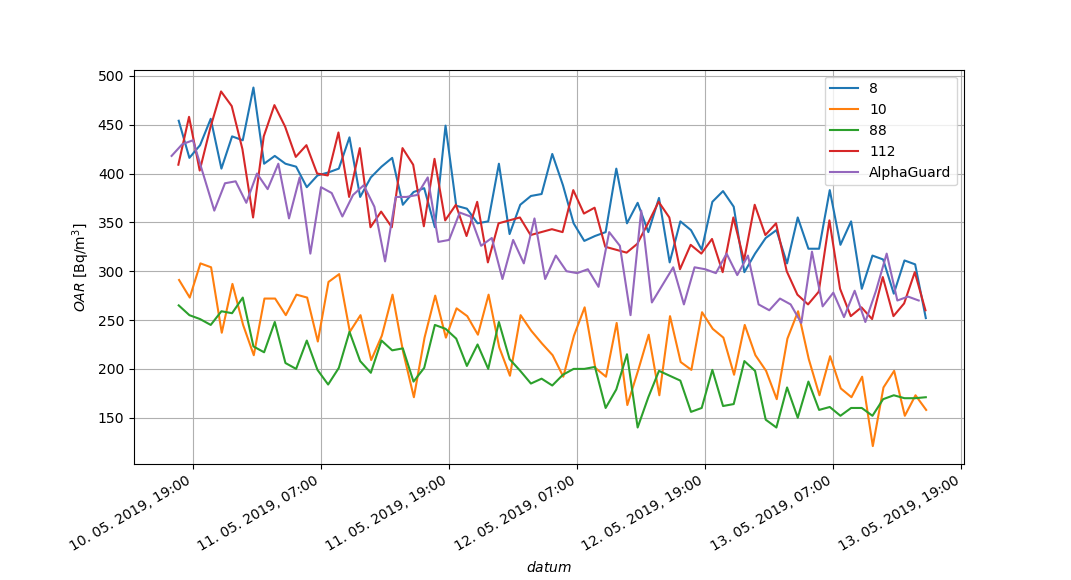
\includegraphics[width=\textwidth]{sondy.png}
		\caption{Vývoj OAR naměřený zkoumanými sondami.}
	\end{figure}
	\begin{table}[ht]
		\centering
		\caption{Statistiky jsou v \si{Bq/m^3}.}
\begin{tabular}{lrrrrrrrr}
	\toprule
	ID sondy &  count &  mean &  std &  min &  25\% &  50\% &  75\% &  max \\
	\midrule
	8          &     71 &   369 &   47 &  252 &  337 &  368 &  405 &  488 \\
	10         &     71 &   228 &   41 &  121 &  198 &  232 &  256 &  308 \\
	88         &     71 &   198 &   33 &  140 &  170 &  198 &  220 &  273 \\
	112        &     71 &   354 &   58 &  251 &  318 &  349 &  399 &  484 \\
	\midrule
	AlphaGuard &     71 &   328 &   50 &  247 &  285 &  318 &  373 &  434 \\
	\bottomrule
\end{tabular}
	\end{table}
\begin{figure}
	\centering
	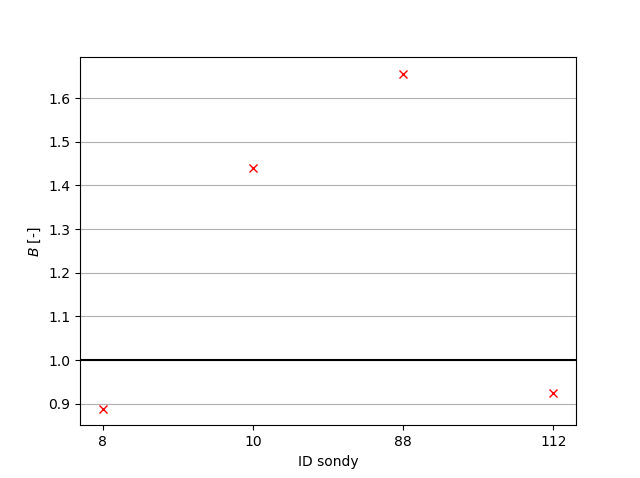
\includegraphics[width=0.7\linewidth]{B}
	\caption{Bulharské konstanty proměřených TESLA sond.}
	\label{fig:B}
\end{figure}

\begin{table}[ht]
\centering
\caption{Bulharské konstanty TESLA sond odvozené od referenčního AlphaGuardu. Skutečná hodnota $OAR$ se vypočte ze vztahu $OAR=B\cdot OAR_T$, kde $OAR_T$ je naměřená obj. aktivita radonu danou TESLA sondou.}
\begin{tabular}{lrr}
	\toprule
	ID sondy &     $B$ &  $u(B)$ \\
	\midrule
	8   & 0.889 &  0.177 \\
	10  & 1.440 &  0.340 \\
	88  & 1.655 &  0.377 \\
	112 & 0.925 &  0.208 \\
	\bottomrule
\end{tabular}
\end{table}
\end{document}